\documentclass[11pt,preprint, authoryear]{elsarticle}

\usepackage{lmodern}
%%%% My spacing
\usepackage{setspace}
\setstretch{1.2}
\DeclareMathSizes{12}{14}{10}{10}

% Wrap around which gives all figures included the [H] command, or places it "here". This can be tedious to code in Rmarkdown.
\usepackage{float}
\let\origfigure\figure
\let\endorigfigure\endfigure
\renewenvironment{figure}[1][2] {
    \expandafter\origfigure\expandafter[H]
} {
    \endorigfigure
}

\let\origtable\table
\let\endorigtable\endtable
\renewenvironment{table}[1][2] {
    \expandafter\origtable\expandafter[H]
} {
    \endorigtable
}


\usepackage{ifxetex,ifluatex}
\usepackage{fixltx2e} % provides \textsubscript
\ifnum 0\ifxetex 1\fi\ifluatex 1\fi=0 % if pdftex
  \usepackage[T1]{fontenc}
  \usepackage[utf8]{inputenc}
\else % if luatex or xelatex
  \ifxetex
    \usepackage{mathspec}
    \usepackage{xltxtra,xunicode}
  \else
    \usepackage{fontspec}
  \fi
  \defaultfontfeatures{Mapping=tex-text,Scale=MatchLowercase}
  \newcommand{\euro}{€}
\fi

\usepackage{amssymb, amsmath, amsthm, amsfonts}

\def\bibsection{\section*{References}} %%% Make "References" appear before bibliography


\usepackage[round]{natbib}

\usepackage{longtable}
\usepackage[margin=2.3cm,bottom=2cm,top=2.5cm, includefoot]{geometry}
\usepackage{fancyhdr}
\usepackage[bottom, hang, flushmargin]{footmisc}
\usepackage{graphicx}
\numberwithin{equation}{section}
\numberwithin{figure}{section}
\numberwithin{table}{section}
\setlength{\parindent}{0cm}
\setlength{\parskip}{1.3ex plus 0.5ex minus 0.3ex}
\usepackage{textcomp}
\renewcommand{\headrulewidth}{0.2pt}
\renewcommand{\footrulewidth}{0.3pt}

\usepackage{array}
\newcolumntype{x}[1]{>{\centering\arraybackslash\hspace{0pt}}p{#1}}

%%%%  Remove the "preprint submitted to" part. Don't worry about this either, it just looks better without it:
\makeatletter
\def\ps@pprintTitle{%
  \let\@oddhead\@empty
  \let\@evenhead\@empty
  \let\@oddfoot\@empty
  \let\@evenfoot\@oddfoot
}
\makeatother

 \def\tightlist{} % This allows for subbullets!

\usepackage{hyperref}
\hypersetup{breaklinks=true,
            bookmarks=true,
            colorlinks=true,
            citecolor=blue,
            urlcolor=blue,
            linkcolor=blue,
            pdfborder={0 0 0}}


% The following packages allow huxtable to work:
\usepackage{siunitx}
\usepackage{multirow}
\usepackage{hhline}
\usepackage{calc}
\usepackage{tabularx}
\usepackage{booktabs}
\usepackage{caption}


\newenvironment{columns}[1][]{}{}

\newenvironment{column}[1]{\begin{minipage}{#1}\ignorespaces}{%
\end{minipage}
\ifhmode\unskip\fi
\aftergroup\useignorespacesandallpars}

\def\useignorespacesandallpars#1\ignorespaces\fi{%
#1\fi\ignorespacesandallpars}

\makeatletter
\def\ignorespacesandallpars{%
  \@ifnextchar\par
    {\expandafter\ignorespacesandallpars\@gobble}%
    {}%
}
\makeatother

\newenvironment{CSLReferences}[2]{%
}

\urlstyle{same}  % don't use monospace font for urls
\setlength{\parindent}{0pt}
\setlength{\parskip}{6pt plus 2pt minus 1pt}
\setlength{\emergencystretch}{3em}  % prevent overfull lines
\setcounter{secnumdepth}{5}

%%% Use protect on footnotes to avoid problems with footnotes in titles
\let\rmarkdownfootnote\footnote%
\def\footnote{\protect\rmarkdownfootnote}
\IfFileExists{upquote.sty}{\usepackage{upquote}}{}

%%% Include extra packages specified by user

%%% Hard setting column skips for reports - this ensures greater consistency and control over the length settings in the document.
%% page layout
%% paragraphs
\setlength{\baselineskip}{12pt plus 0pt minus 0pt}
\setlength{\parskip}{12pt plus 0pt minus 0pt}
\setlength{\parindent}{0pt plus 0pt minus 0pt}
%% floats
\setlength{\floatsep}{12pt plus 0 pt minus 0pt}
\setlength{\textfloatsep}{20pt plus 0pt minus 0pt}
\setlength{\intextsep}{14pt plus 0pt minus 0pt}
\setlength{\dbltextfloatsep}{20pt plus 0pt minus 0pt}
\setlength{\dblfloatsep}{14pt plus 0pt minus 0pt}
%% maths
\setlength{\abovedisplayskip}{12pt plus 0pt minus 0pt}
\setlength{\belowdisplayskip}{12pt plus 0pt minus 0pt}
%% lists
\setlength{\topsep}{10pt plus 0pt minus 0pt}
\setlength{\partopsep}{3pt plus 0pt minus 0pt}
\setlength{\itemsep}{5pt plus 0pt minus 0pt}
\setlength{\labelsep}{8mm plus 0mm minus 0mm}
\setlength{\parsep}{\the\parskip}
\setlength{\listparindent}{\the\parindent}
%% verbatim
\setlength{\fboxsep}{5pt plus 0pt minus 0pt}



\begin{document}



\begin{frontmatter}  %

\title{Settling the Debate: The GOAT of tennis}

% Set to FALSE if wanting to remove title (for submission)




\author[Add1]{Grace Grant - 21653488}
\ead{21653488@sun.ac.za}





\address[Add1]{Stellenbosch University, Stellenbosch, South Africa}



\vspace{1cm}





\vspace{0.5cm}

\end{frontmatter}

\setcounter{footnote}{0}



%________________________
% Header and Footers
%%%%%%%%%%%%%%%%%%%%%%%%%%%%%%%%%
\pagestyle{fancy}
\chead{}
\rhead{}
\lfoot{}
\rfoot{}
\lhead{}
%\rfoot{\footnotesize Page \thepage } % "e.g. Page 2"
\cfoot{}

%\setlength\headheight{30pt}
%%%%%%%%%%%%%%%%%%%%%%%%%%%%%%%%%
%________________________

\headsep 35pt % So that header does not go over title




\hypertarget{introduction}{%
\section{\texorpdfstring{Introduction
\label{Introduction}}{Introduction }}\label{introduction}}

The Open Era of tennis has seen the world's greatest players and some of
the most riveting and exceptional performances in big events. Players
such as Rod Laver, John McEnroe, Ivan Lendl and Pete Sampras made a name
for themselves over the course of their careers but it is arguably the
Big 3 - Roger Federer, Rafael Nadal and Novak Djokovic - who have
captured the world's attention and have elevated the sport beyond
anything seen before. The following machine learning project thus aims
to predict which of these men should be considered the GOAT - the
greatest of all time. I make use of a random forest model applied to a
dataset containing all the matches in the main ATP tour events from
2003, when Federer won his first Grand Slam. However, I first provide
descriptive statistics to better understand the nature of the data as
well as to gain insight into the Big 3's performance.

\hypertarget{descriptive-statistics}{%
\section{Descriptive statistics}\label{descriptive-statistics}}

These descriptive statistics make use of the ATP data from 1968, the
start of the Open Era, before focusing on the current period with Nadal,
Federer and Djokovic. I have chosen to first look at the top Grand Slam
wins over time, choosing the players with top 10 most titles. Number of
Grand Slams is the most commonly used metric in the debate of the best
player and can thus be used to understand which players in the Open Era
gained recognition for their performances. The following graph
highlights this, showing the top 10 Grand Slam winners from 1968 to
2022.

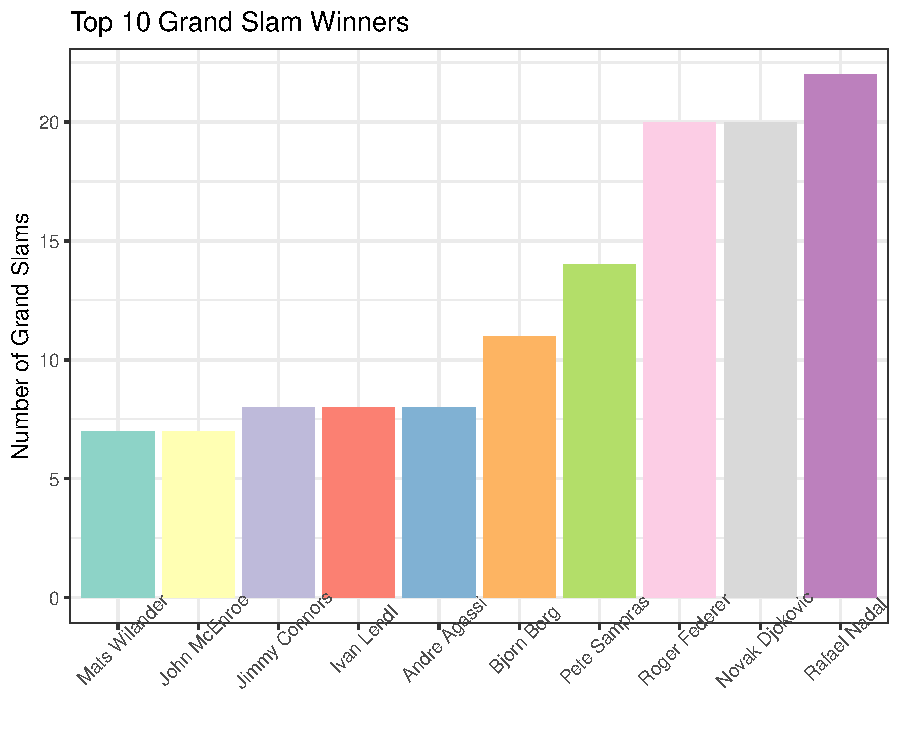
\includegraphics{Write-up_files/figure-latex/GS winners-1.pdf}

This graph illustrates the dominance of the Big 3 in Grand Slam wins,
with Nadal holding the most titles at 22 as of 2022. The other seven
players in the graph, who also had illustrious careers, lag quite far
behind Nadal, Federer and Djokovic. Pete Sampras, for example, who was
still competing when Federer began his career, only has 14 Grand Slams
to his name while the other players have even fewer. This shows how the
Big 3 have elevated the level of the game and raised the bar for what is
considered high-level achievement.

The following table further supports the Big 3's supremacy, showing the
winners of each Grand Slam from 2003 to 2019.

\begin{table}[ht]
\centering
\begin{tabular}{rlllll}
  \hline
 & year & Australian Open & Roland Garros & Wimbledon & US Open \\ 
  \hline
1 & 2003 & Andre Agassi & Juan Carlos Ferrero & Roger Federer & Andy Roddick \\ 
  2 & 2004 & Roger Federer & Gaston Gaudio & Roger Federer & Roger Federer \\ 
  3 & 2005 & Marat Safin & Rafael Nadal & Roger Federer & Roger Federer \\ 
  4 & 2006 & Roger Federer & Rafael Nadal & Roger Federer & Roger Federer \\ 
  5 & 2007 & Roger Federer & Rafael Nadal & Roger Federer & Roger Federer \\ 
  6 & 2008 & Novak Djokovic & Rafael Nadal & Rafael Nadal & Roger Federer \\ 
  7 & 2009 & Rafael Nadal & Roger Federer & Roger Federer & Juan Martin del Potro \\ 
  8 & 2010 & Roger Federer & Rafael Nadal & Rafael Nadal & Rafael Nadal \\ 
  9 & 2011 & Novak Djokovic & Rafael Nadal & Novak Djokovic & Novak Djokovic \\ 
  10 & 2012 & Novak Djokovic & Rafael Nadal & Roger Federer & Andy Murray \\ 
  11 & 2013 & Novak Djokovic & Rafael Nadal & Andy Murray & Rafael Nadal \\ 
  12 & 2014 & Stan Wawrinka & Rafael Nadal & Novak Djokovic & Marin Cilic \\ 
  13 & 2015 & Novak Djokovic & Stan Wawrinka & Novak Djokovic & Novak Djokovic \\ 
  14 & 2016 & Novak Djokovic & Novak Djokovic & Andy Murray & Stan Wawrinka \\ 
  15 & 2017 & Roger Federer & Rafael Nadal & Roger Federer & Rafael Nadal \\ 
  16 & 2018 & Roger Federer & Rafael Nadal & Novak Djokovic & Novak Djokovic \\ 
  17 & 2019 & Novak Djokovic & Rafael Nadal & Novak Djokovic & Rafael Nadal \\ 
   \hline
\end{tabular}
\caption{Grand Slam Winners Since 2003} 
\end{table}

This is evidence of the extent to which Nadal, Federer and Djokovic have
dominated the Grand Slam circuit. Since 2003, when Federer won his first
Grand Slam, the Big 3 have won 55 out of the 68 tournaments in this
period, with only Andy Murray and Stan Wawrinka winning more than one
each of all the other players. There is therefore no doubt that these
top 3 players will rival each other as being the greatest of all time.

Beyond showing Grand Slam wins, the data also provides additional
information on the statistics of each match played relating to length of
the game, serving and break points statistics and the surface of the
tournament among others. The following tables and figures illustrate how
each of the Big 3's wins are broken down and relate to some of these
variables.

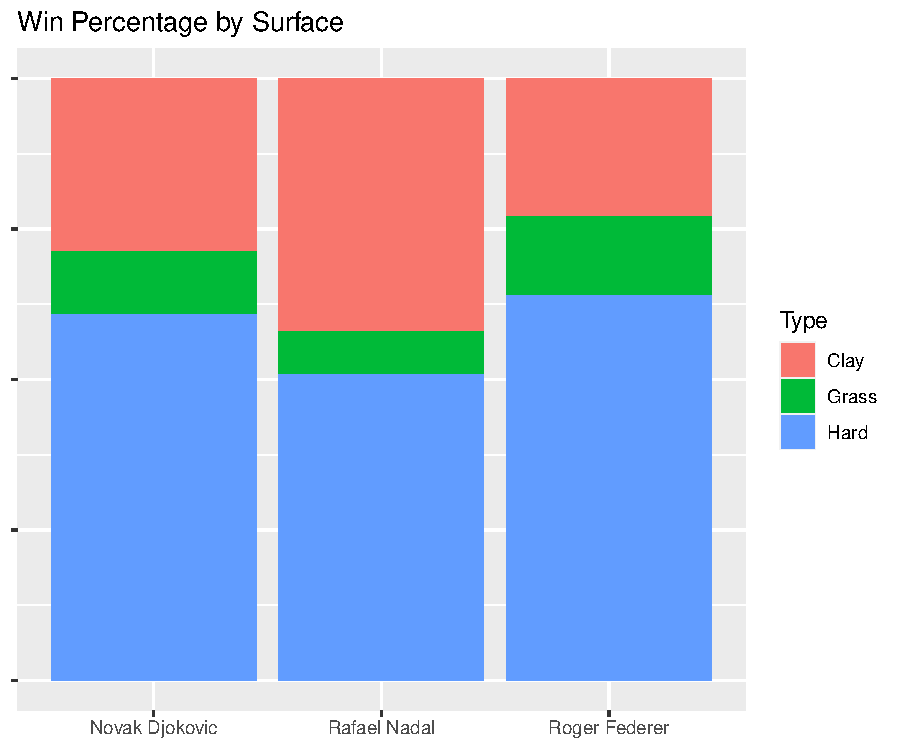
\includegraphics{Write-up_files/figure-latex/more descriptive-1.pdf}

These graphs, referencing surfaces by their colour, show each of Nadal,
Federer and Djokovic's win percentages on each surface. This indicates
that Nadal has a much higher win record on clay than the other two,
confirming his status as the King of Clay. All players have the highest
win records on hard court, which may partly link to this being the
surface with the most number of matches, but Federer and Djokovic have a
more even split across surfaces, indicating their versatility.

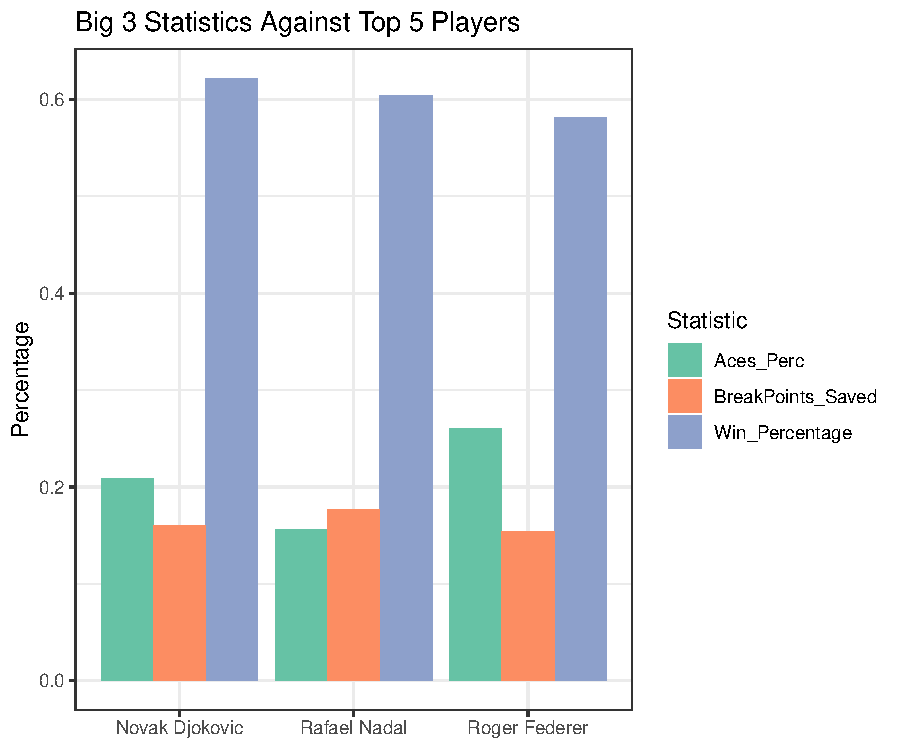
\includegraphics{Write-up_files/figure-latex/grouped bar-1.pdf}

The grouped chart sheds further light into each of the Big 3's
statistics against top 5 players, averaging across matches. Djokovic has
the highest win percentage, Nadal the highest breakpoints saved and
Federer the highest ace percentage. Federer is known to have a strong
serve that is difficult to read so it is understandable that his ace
percentage is higher than the others, while Nadal is known to fight back
when he is at a disadvantage, hence the high breakpoints saved. However,
I would argue that win percentage is the most important statistic to
consider because this relates directly to number of wins and titles.
This graph shows that Djokovic has the best record against top 5 players
in the main ATP events, winning approximately 62 percent of his matches.

\begin{table}[ht]
\centering
\begin{tabular}{rlr}
  \hline
 & Player & TTaken \\ 
  \hline
1 & Rafael Nadal & 125.00 \\ 
  2 & Roger Federer & 109.00 \\ 
  3 & Novak Djokovic & 121.00 \\ 
   \hline
\end{tabular}
\caption{Average Time Taken} 
\end{table}

This final table provides an overview of the Big 3's average match times
across all games. Roger Federer is shown to take the least amount of
time to finish matches, averaging at 109 minutes or approximately 1 hour
and 45 minutes. This is quite significantly different from Nadal and
Djokovic, suggesting that Federer prefers a shorter game format. This
may link to his playing style which involves big serves and net play
which generally induces shorter matches due to less rallies.

These graphs and tables provide a sufficient overview of player
performance and offers a comparison of the Big 3'\,'s results and more
specifics of their playing style and outcomes. However, to obtain a more
definitive answer to the question of the GOAT, I make use of a random
forest model which is discussed and interpreted in the next sections.

\hypertarget{data-and-methodology}{%
\section{Data and methodology}\label{data-and-methodology}}

I have made use of a dataset that includes all the ATP matches from 1968
to 2022, within which is included match and player statistics. I merged
these documents and filtered the data frame to include only main tour
events i.e.~Grand Slams, Masters and Tour Finals. These are the most
important events in the tennis circuit and the ones in which the top
players participate the most. I further subset the data to include
matches from 2003, when Roger Federer won his first Grand Slam at
Wimbledon. This allows me to focus on the time period of the Big 3 who
are at the centre of the debate surrounding the GOAT. There is also a
large amount of missing information in earlier dates, particularly in
the 1960s, 70s and 80s, so subsetting to start at 2003 avoids issues
related to NA values. Finally, I selected the features I deemed most
relevant to my model to arrive at the final data frame. These features
included tournament names and surfaces, player characteristics - such as
their height and age - and various match statistics linked to time
taken, breakpoints faced and saved, aces and first serves in. These
features were included for both the winner and the loser of each match.
Additional feature engineering involved turning categorical variables,
such as surface, into factors to ensure the model accurately processed
the data.

Lastly, I had to perform target engineering to establish an outcome
variable to use for predictions in the model. I created a random binary
variable and assigned the winner and loser of each game to player 1 and
player 2 based on the random binary variable. This ensured that the new
match winner column had an even split between player 1 winning or losing
each match and could be used as the target variable.

\hypertarget{the-random-forest-model}{%
\subsection{The random forest model}\label{the-random-forest-model}}

I made use of a random forest model model to process my data and perform
predictions. Random forests are extensions or modifications of bagged
decision trees and build a series of de-correlated trees to improve
predictive performance. They have become a popular out-of-the-box
learning algorithm because they enjoy good predictive performance and
require minimal hyperparameter tuning
(\protect\hyperlink{ref-boehmke2019hands}{Boehmke \& Greenwell, 2019}).
My model had 19 features with a binary target variable, making it a
classification problem. I constructed two random forest models, a
baseline model using the default hyperparameters as outlined by Boehmke
\& Greenwell (\protect\hyperlink{ref-boehmke2019hands}{2019}) and a
second model based on the hyperparamater tuning done via a grid search.
The predictions from the hypertuned model as well as its accuracy
measures are presented and discussed below, including comparisons with
the default model.

\hypertarget{results-and-discussion}{%
\section{Results and discussion}\label{results-and-discussion}}

The following table shows the predictions from my hypertuned model,
indicating that Roger Federer is the GOAT based on win percentage.
Djokovic and Nadal follow closely behind, while Andy Murray and Gael
Monfils have the fourth and fifth highest win percentages, respectively.

\begin{verbatim}
## [1] 0.3038952
\end{verbatim}

\begin{table}[ht]
\centering
\begin{tabular}{rlrr}
  \hline
 & Player & win\_percentage & win\_count \\ 
  \hline
1 & Roger Federer & 0.89 & 110 \\ 
  2 & Novak Djokovic & 0.88 & 108 \\ 
  3 & Rafael Nadal & 0.86 & 107 \\ 
  4 & Andy Murray & 0.84 &  67 \\ 
  5 & Gael Monfils & 0.82 &  45 \\ 
   \hline
\end{tabular}
\caption{The Best of Tennis} 
\end{table}

The model produces results that make sense. The Big 3 are the top three
highest performers, while Andy Murray (who has sometimes been grouped
into the Big 4 category) is in fourth place. I was surprised to see Gael
Monfils finish in fifth place given that he has never won a major but
the data set looks at matches across all main ATP events which could
point to why he appears in the top winners.

Although the results make intuitive sense, it is also necessary to test
the predictive performance of the model to see how accurate these
predictions are based on the data. I compare the accuracy, sensitivity
and specificity of the baseline and tuned models to highlight their
predictive performance.

\begin{table}[ht]
\centering
\begin{tabular}{rlrrr}
  \hline
 & Model & Accuracy & Sensitivity & Specificity \\ 
  \hline
1 & Baseline model & 0.92 & 0.93 & 0.91 \\ 
  2 & Tuned model & 0.92 & 0.92 & 0.91 \\ 
   \hline
\end{tabular}
\caption{Accuracy Across the Baseline and Tuned Models} 
\end{table}

This table, firstly, shows that both models have high and almost
identical results across the accuracy measures. This could be due to the
fact that the tuned model has very similar hyperparameters to the
default model. The best model, as determined by the grid search, is
given below.

\begin{table}[ht]
\centering
\begin{tabular}{rrrlrrr}
  \hline
 & mtry & min.node.size & replace & sample.fraction & rmse & perc\_gain \\ 
  \hline
1 & 4.00 & 1.00 & FALSE & 0.63 & 0.30 & 2.73 \\ 
   \hline
\end{tabular}
\caption{Grid Search Results} 
\end{table}

The mtry and node size hyperparameters determined by the grid search are
the same as those in the baseline model and both models also have the
same number of trees (500). This could account for the similarity in
results. The actual values in the table indicate that the model is
highly accurate and predicts the data well. The sensitivity shows that
the model predicts successes (i.e.~player 1 winning) correctly 92
percent of the time and predicts failures (player 1 losing) correctly 90
percent of the time.

An additional evaluation of the model considers errors within the random
forest. One metric is the Out-of-Bag (OOB) prediction error which is
calculated by evaluating the predictions of each tree on the out-of-bag
samples that were not used during training
(\protect\hyperlink{ref-boehmke2019hands}{Boehmke \& Greenwell, 2019}).
The RMSE, which is just the squareroot of the OOB prediction error, is
another useful metric to understand the model's errors. The following
output shows the errors from the baseline model and the tuned model.

\begin{table}[ht]
\centering
\begin{tabular}{rlrr}
  \hline
 & Model & OOB & RMSE \\ 
  \hline
1 & Baseline model & 9.24 & 30.39 \\ 
  2 & Tuned model & 8.66 & 29.56 \\ 
   \hline
\end{tabular}
\caption{Errors Across the Baseline and Tuned Models in Percent} 
\end{table}

These results show that the tuned model performs slightly better than
the baseline, with a lower OOB prediction error and RMSE. This indicates
that the tuned model is a better predictive model.

\hypertarget{feature-importance}{%
\subsection{Feature importance}\label{feature-importance}}

The final element of evaluating the random forest is assessing the
feature importance using both the impurity and permutation measures. The
impurity-based measure bases feature importance on how much each feature
contributes to reducing impurity when making splits in the trees.
Permutation-based feature importance, on the other hand, measures how
much the accuracy of the model deteriorates when the values of a feature
are randomly shuffled. Both are necessary to determine the ranking of
each feature's importance in the model.

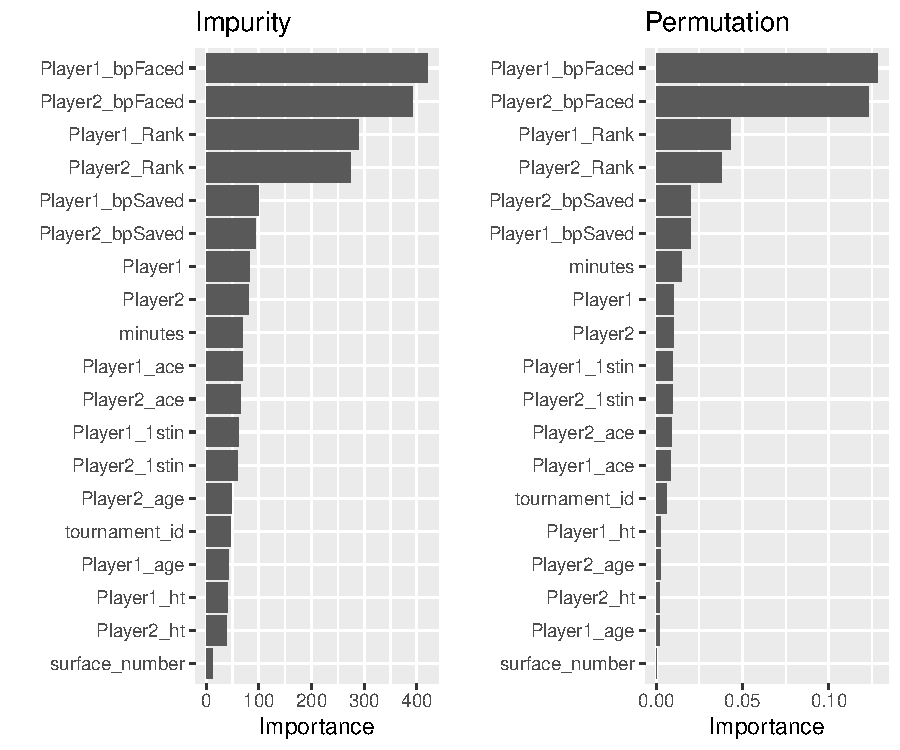
\includegraphics{Write-up_files/figure-latex/feature importance-1.pdf}

Both feature importance graphs indicate that breakpoints faced, rank and
breakpoints saved are the most important features in predicting the
match winner. This makes sense as, understandably, higher ranked players
generally win more matches, while breakpoints are highly important in
tennis matches. Players gain advantage by breaking their opponents
service games which is normally directly correlated with winning
matches. These graphs therefore align with general tennis practice.

\hypertarget{conclusion}{%
\section{Conclusion}\label{conclusion}}

This machine learning model provided an accurate prediction of who the
best tennis players of this generation are. I used a random forest
trained on a dataset consisting of all the ATP matches in the main
events from 2003 to 2019. Based on this model, I predict Roger Federer
to be the greatest of all time. However, there are two caveats to this
conclusion. Firstly, the data only runs to 2019 which does not take into
account the most recent events in tennis i.e.~Novak Djokovic winning his
23rd Grand Slam at the 2023 Roland Garros. Because of this feat, many
are hailing him as the GOAT. Additionally, I have only 19 features in my
model, relating to player characteristics and match statistics. To say
someone is a great player goes beyond these metrics - popularity on and
off the court, viewership, prize-money and many other factors also play
a contributing role. As a Federer fan, I am very pleased with the
results of the model but it is very difficult to settle the debate of
the GOAT of tennis. Each of the Big 3 - Nadal, Djokovic and Federer -
have achieved exceptional results and will be considered the greatest
players of this generation and the greatest players of all time.

\hypertarget{refs}{}
\begin{CSLReferences}{1}{0}
\leavevmode\vadjust pre{\hypertarget{ref-boehmke2019hands}{}}%
Boehmke, B. \& Greenwell, B.M. 2019. \emph{Hands-on machine learning
with r}. CRC press.

\end{CSLReferences}

\bibliography{Tex/ref}





\end{document}
